\documentclass[12pt,a4paper]{article}
\usepackage[latin1]{inputenc}
\usepackage{amsmath}
\usepackage{amsfonts}
\usepackage{amssymb}
\usepackage{graphicx}
\author{Neil Armand Bantoc and James Carlo Plaras}
\title{Galaxhoot User Manual}
\date{}
\begin{document}
\maketitle
\section{System Requirements}
Device with:
\begin{itemize}
\item Android OS 1.6 or higher
\item OpenGL ES 2.0 or higher
\item Built-in Accelerometer
\end{itemize}

\section{Installation}

\begin{enumerate}
\item Copy Galaxhoot.apk on your phone
\item Install the app by opening the apk using the file manager of your choice.
\item Launch the Game!
\end{enumerate}

\newpage
\section{Game Instructions}
\subsection{How to play}
Move your spaceship to the left by moving your device to the left and to the right by moving it to the right. You may also change view mode depending on where you are comfortable. The spaceship will automatically fire its guns once it has finished its reloading time. Hit them all and don't be hit. Aim for the highest score and boast it to your friends. ENJOY!

\subsection{In-Game User Interface}
\begin{figure}[h]
\centering 
  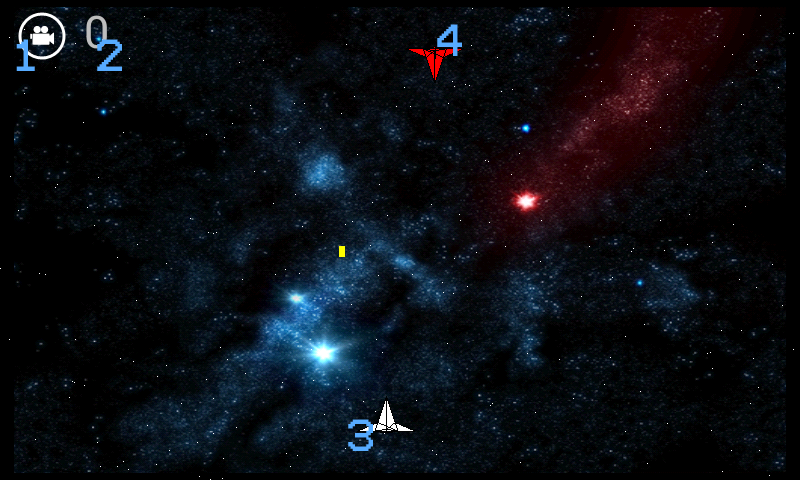
\includegraphics[height=70mm]{images/UILayout.png}
  \caption{In-game layout}
\end{figure}

\begin{figure}[h]
\centering 
  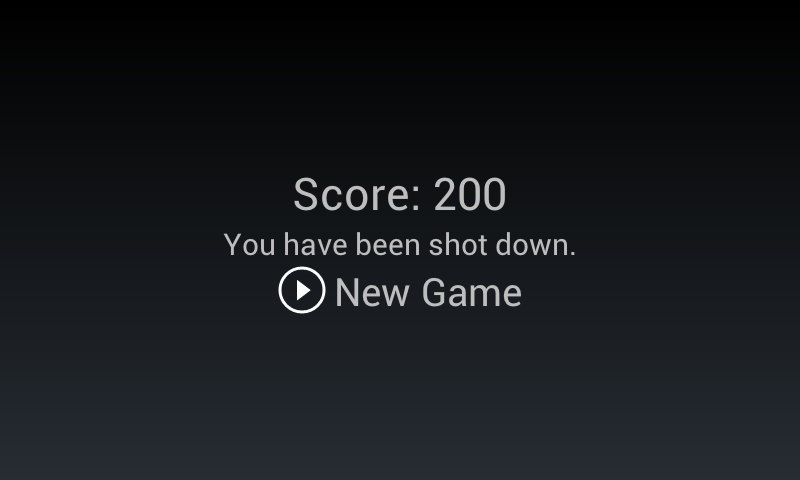
\includegraphics[height=70mm]{images/gameover.png}
  \caption{Game over screen}
\end{figure}

\begin{enumerate}
\item \textbf{Change View Button}\\
Triggers the change of view mode in the game
\item \textbf{Score/Message Section}\\
Displays your current score. Also displays some in-game messages.
\item \textbf{Main Ship}\\
This is the ship you control.
\item \textbf{Enemy Ship}\\
Enemy Ships are red in color.
\end{enumerate}


\newpage
\subsection{View Modes}
\begin{figure}[h]
\centering 
  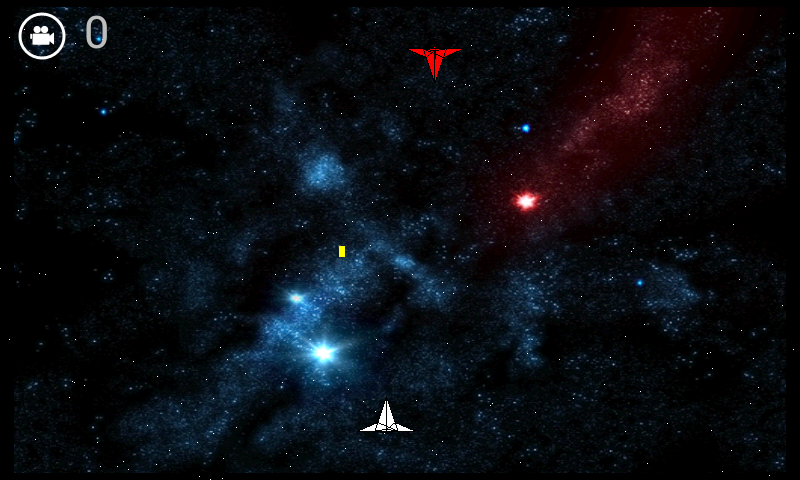
\includegraphics[height=65mm]{images/topview.png}
  \caption{Birds Eye View}
\end{figure}

\begin{figure}[h]
\centering 
  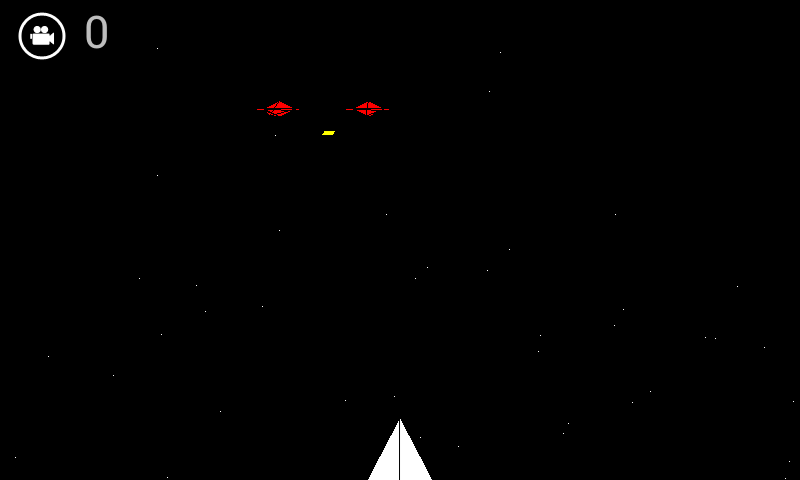
\includegraphics[height=65mm]{images/1stpersonview.png}
  \caption{First Person View}
\end{figure}
\newpage
\begin{figure}[h]
\centering 
  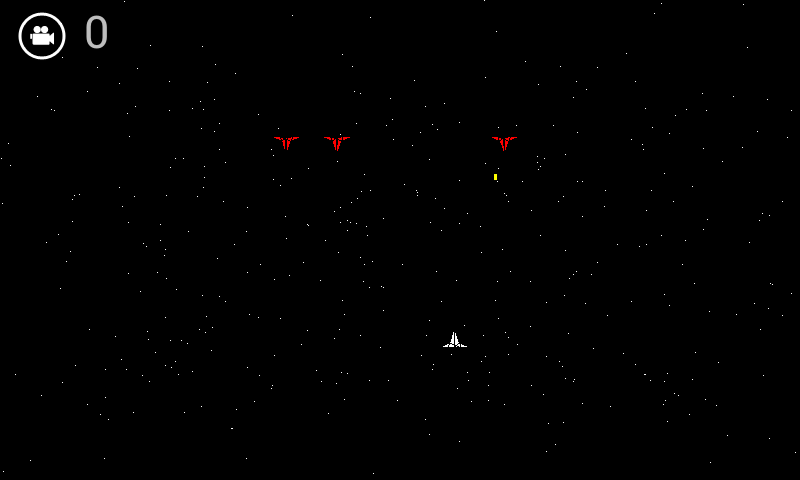
\includegraphics[height=65mm]{images/3Dview.png}
  \caption{3D View}
\end{figure}



\newpage
\section{Extension}
You may continue to develop \textbf{GALAXHOOT}. The source code is available at the \textit{source} folder. It contains the \textit{Galaxhoot} folder which is a Eclipse Android Project.

\subsection{Development Requirements}
\begin{itemize}
\item Android SDK 1.6 or higher and platform-tools
\item Eclipse ADT plugin
\item Developement Device (optional)
\end{itemize}
\subsection{Development Resources}
For more information on Android Open GL development visit the following sites:
\begin{itemize}
\item Android Development Overview
\\http://developer.android.com/guide/index.html
\item Android SDK Installation
\\http://developer.android.com/sdk/installing.html
\item OpenGL ES Introduction \\ http://developer.android.com/guide/topics/graphics/opengl.html
\end{itemize}
\end{document}